% $HeadURL: https://sbgn.svn.sourceforge.net/svnroot/sbgn/ProcessDiagram/tags/L1V1.3Full/sources/macromolecule.tex $

\subsection{Glyph: \glyph{Macromolecule}}
\label{sec:macromolecule}

Many biological processes involve \emph{macromolecules}: biochemical substances that are built up from the covalent linking of pseudo-identical units.  Examples of macromolecules include proteins, nucleic acids (RNA, DNA), and polysaccharides (glycogen, cellulose, starch, etc.).  Attempting to define a separate glyph for all of these different molecules would lead to an explosion of symbols in SBGN, so instead, \SBGNPDLone defines only one glyph for all macromolecules.  The same glyph is to be used for a protein, a nucleic acid, a complex sugar, and so on.  The exact nature of a particular macromolecule in a map is then clarified using its label and decorations, as will become clear below.  A \glyph{macromolecule} is represented by a rectangular container with rounded corners, as illustrated in \fig{macromolecule}. 

\begin{figure}[H]
  \centering
  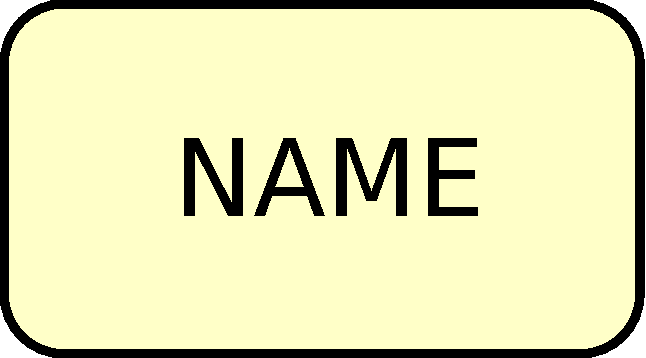
\includegraphics[width = 1.25in]{images/macromolecule-plain}
  \caption{The \PD glyph for \glyph{macromolecule}.}
  \label{fig:macromolecule}
\end{figure}

Examples of \glyph{macromolecules} are presented in \fig{macromolecule-examples}.

\begin{figure}[H]
  \centering
  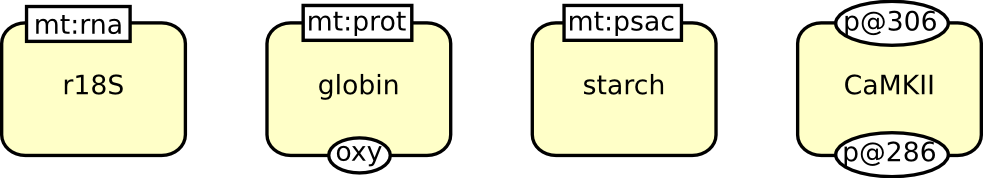
\includegraphics[scale = 0.5]{images/macromolecule-examples}
  \caption{Examples of \glyph{macromolecules}. From left to right: the macromolecule of 18S ribosomal RNA, globin (a protein) in the oxygenated state, a molecule of starch (polymer of glucose), calcium calmodulin kinase 2 phosphorylated on threonine 286 and 306.}
  \label{fig:macromolecule-examples}
\end{figure}




% The following is for [X]Emacs users.   Please leave in place.
% Local Variables:
% TeX-master: "../sbgn_PD-level1"
% End:
